%9/98
\documentclass[12pt]{article}
\pagestyle{empty}

%\input amssym.def
%\input amssym
%\input psfig.tex
%\input mssymb
\usepackage{amsmath} 
\usepackage{graphicx}
%%\usepackage{showlabels}
%\renewcommand\marginpar[1]{}
%\newcommand{\comment}[1]{}
\textwidth 6in
\oddsidemargin 0.25in
\topmargin -0.75in
\textheight 8.5in




\newcommand{\CourseName}{\textsf{MATH 6480 - John Haman }}
\begin{document}
\medskip
\begin{flushleft}
  \CourseName \hfill \textsf{Homework 1}\\
\medskip





\begin{enumerate}

\item 1.5 
\begin{enumerate}

\item Let $n = 17$ and $x = 13$. Then the p-value is $2*P(X\geq13|p=1/2) =2*P(X\leq 4|p=1/2) $ 

\begin{verbatim}
> 2*pbinom(4,17,0.5)
[1] 0.04904175
\end{verbatim}

\item Stage 1 : $n_1 = 17$, Reject if $X_1 \geq 13 $ or $X_1 \leq 4$. Stage 2: $n_2 = 27$. Reject if $X_1 + X_2 \geq 29 $ or $x_1 + X_2 \leq 15$.

Let $X_1 = 13$.

Then p-value = $2*P(X_1 \geq 13| p=1/2) + 2*P(X_1 + X_2 \leq 15 \,\, \textrm{and} \,\, 5 \leq X_1 \leq 12 | p = 1/2) = 0.049 + \sum_{i=5}^{12} P( X_2 \leq 15 - X_i | X_1 = i)*P(X_1 = i)$ 

where the last equality follows from an application of Bayes Theorem over of a set of disjoint events. 

\begin{verbatim}
> for (i in 5:12){
+ 
+     s[i] <- pbinom(15-i,27,0.5) * dbinom(i,17,0.5)
+     }
>     prob <- sum(s);prob
[1] 0.01794216
>     prob <-2* sum(s);prob
[1] 0.03588431
> pvalue <- prob + 0.049;pvalue
[1] 0.08488431
\end{verbatim}

The pvalue is $0.0848$.

\item The pvalue will continue to increase as more stages are added to the test. This is clear because with each additional stage, the practitioner gains an addition attempt to accept the null hypothesis. The pvalue will actually approach $1$ since we will pick up an additional amount of ``rejection probability'' with each stage, but the amount will diminish with each added stage, as in part (b), making it impossible to reject the null hypothesis.

\item If a trial is stopped due to allergic reactions, then one needs to first consider whether it is ethical to administer the trial in the first place. Under the frquentist scheme, the pvalue for a stopped experiment such as the one in this example cannot be computed, so the experiment may be discarded and performed again (hopefully without an allergic reaction). Under the Bayesian scheme, it may be possible to perform inferences on a stopped experiment, as we saw in the Binomial vs Negative Binomial example. 

\item I don't think anyone has ever held the pvalue to be objective evidence. To a frequentist, the pvalue may be enough to make a decision in the face of uncertainty, but clearly there is a limitation on its use. Fisher never intended the pvalue to be the basis on which practitioners make test decisions. Hence, pvalues may be abused or misused, but they still have an important place in statistics as long as we understand their assumptions and limitations.

\end{enumerate}

\item  In the Normal - Normal example, let $\sigma^2 = 2$, $\mu = 0$, and $\tau^2 = 2$.

\begin{enumerate}

\item  Suppose $y=4$. Then $B = \frac{\sigma^2}{\sigma^2 + \tau^2} = 1/2$. So $\mathrm{E}(\theta | Y) = B\mu + (1-B)y = \frac{1}{2} * 0 + \frac{1}{2}*4 = 2$. $\mathrm{Var}(\theta | Y ) = \frac{1}{2} * 2 = 1$. 

And a plot of the densities:

\begin{center}
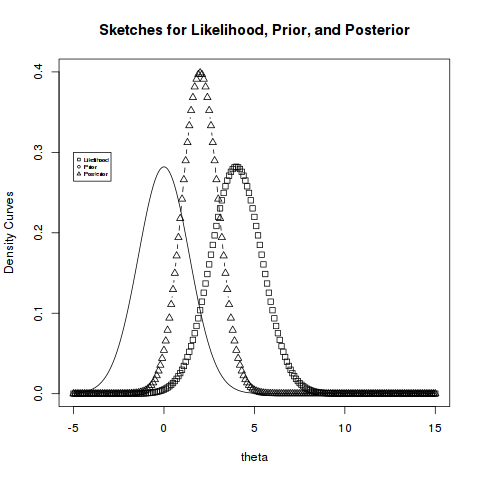
\includegraphics[scale=0.6]{plot1.png}
\end{center}

\item Now let $\sigma^2 = 2$, $\mu = 0$, and $\tau^2 = $, $y=4$. Then $B = \frac{\sigma^2}{\sigma^2 + \tau^2} = 1/10$. So $\mathrm{E}(\theta | Y) = B\mu + (1-B)y = \frac{1}{10} * 0 + \frac{9}{10}*4 = 3.6$. $\mathrm{Var}(\theta | Y ) = \frac{9}{10} * 2 = 1.8$. 

And the plot of the densities:

\begin{center}
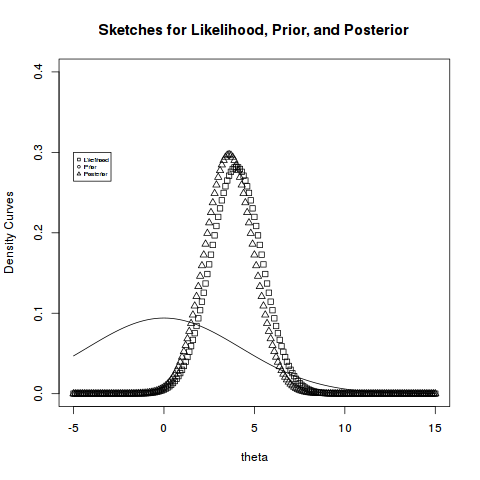
\includegraphics[scale=0.6]{plot2.png}
\end{center}

So when $\tau$ is large, there is the prior is less informative. So a frequentist would prefer $\tau$ to be large.


\end{enumerate}

\item Find the MSE of the estimator $\hat{\theta}_{Bayes} = \frac{Y+1}{n+2}$. 




\begin{equation} 
\begin{split}
\mathrm{MSE}(\hat{\theta}_{Bayes} ) & = \mathrm{Var} (\hat{\theta}_{Bayes} + ( \mathrm{E} (\hat{\theta}_{Bayes} - \theta) ) ^2\\
 & =  \mathrm{Var} (\frac{Y+1}{n+2}) + ( \mathrm{E} (\frac{Y+1}{n+2}) - \theta) ) ^2\\
&= \frac{1}{(n+2)^2} \mathrm{Var} (Y) + (\frac{1}{n+2} \mathrm{E} (Y+1) - \theta)^2 \\
&= \frac{1}{n+2} n \theta (1- \theta) + ( \frac{1}{n+2} (n \theta +1 ) - \theta)^2 \\
&= \frac{n \theta (1- \theta)}{(n+2)^2} + (\frac{n \theta + 1 -\theta(n+2)}{n+2})^2\\
&= \frac{n \theta (1- \theta)}{(n+2)^2} + \frac{(1 - 2 \theta)^2}{(n+2)^2}\\
&= \frac{1 + (n-4)\theta + (4-n)\theta^2}{(n+2)^2}
\end{split}
\end{equation}

One may prefer this estimator if we have some reasonably good information to place a prior distribution on the distribution of $\theta$. On the other hand, if $M$ is small (so there is not much information in the prior), we may prefer the MLE for $\theta$ instead. In this example $M=2$ and $\mu = 1/2$, so in fact the prior density is a uniform distribution, which is not informative. One may compare the MSE of the Bayes estimator to that of the MLE to determine for which estimator is preferable






\end{enumerate}
\end{flushleft}
\end{document}
